\documentclass[1p]{elsarticle_modified}
%\bibliographystyle{elsarticle-num}

%\usepackage[colorlinks]{hyperref}
%\usepackage{abbrmath_seonhwa} %\Abb, \Ascr, \Acal ,\Abf, \Afrak
\usepackage{amsfonts}
\usepackage{amssymb}
\usepackage{amsmath}
\usepackage{amsthm}
\usepackage{scalefnt}
\usepackage{amsbsy}
\usepackage{kotex}
\usepackage{caption}
\usepackage{subfig}
\usepackage{color}
\usepackage{graphicx}
\usepackage{xcolor} %% white, black, red, green, blue, cyan, magenta, yellow
\usepackage{float}
\usepackage{setspace}
\usepackage{hyperref}

\usepackage{tikz}
\usetikzlibrary{arrows}

\usepackage{multirow}
\usepackage{array} % fixed length table
\usepackage{hhline}

%%%%%%%%%%%%%%%%%%%%%
\makeatletter
\renewcommand*\env@matrix[1][\arraystretch]{%
	\edef\arraystretch{#1}%
	\hskip -\arraycolsep
	\let\@ifnextchar\new@ifnextchar
	\array{*\c@MaxMatrixCols c}}
\makeatother %https://tex.stackexchange.com/questions/14071/how-can-i-increase-the-line-spacing-in-a-matrix
%%%%%%%%%%%%%%%

\usepackage[normalem]{ulem}

\newcommand{\msout}[1]{\ifmmode\text{\sout{\ensuremath{#1}}}\else\sout{#1}\fi}
%SOURCE: \msout is \stkout macro in https://tex.stackexchange.com/questions/20609/strikeout-in-math-mode

\newcommand{\cancel}[1]{
	\ifmmode
	{\color{red}\msout{#1}}
	\else
	{\color{red}\sout{#1}}
	\fi
}

\newcommand{\add}[1]{
	{\color{blue}\uwave{#1}}
}

\newcommand{\replace}[2]{
	\ifmmode
	{\color{red}\msout{#1}}{\color{blue}\uwave{#2}}
	\else
	{\color{red}\sout{#1}}{\color{blue}\uwave{#2}}
	\fi
}

\newcommand{\Sol}{\mathcal{S}} %segment
\newcommand{\D}{D} %diagram
\newcommand{\A}{\mathcal{A}} %arc


%%%%%%%%%%%%%%%%%%%%%%%%%%%%%5 test

\def\sl{\operatorname{\textup{SL}}(2,\Cbb)}
\def\psl{\operatorname{\textup{PSL}}(2,\Cbb)}
\def\quan{\mkern 1mu \triangleright \mkern 1mu}

\theoremstyle{definition}
\newtheorem{thm}{Theorem}[section]
\newtheorem{prop}[thm]{Proposition}
\newtheorem{lem}[thm]{Lemma}
\newtheorem{ques}[thm]{Question}
\newtheorem{cor}[thm]{Corollary}
\newtheorem{defn}[thm]{Definition}
\newtheorem{exam}[thm]{Example}
\newtheorem{rmk}[thm]{Remark}
\newtheorem{alg}[thm]{Algorithm}

\newcommand{\I}{\sqrt{-1}}
\begin{document}

%\begin{frontmatter}
%
%\title{Boundary parabolic representations of knots up to 8 crossings}
%
%%% Group authors per affiliation:
%\author{Yunhi Cho} 
%\address{Department of Mathematics, University of Seoul, Seoul, Korea}
%\ead{yhcho@uos.ac.kr}
%
%
%\author{Seonhwa Kim} %\fnref{s_kim}}
%\address{Center for Geometry and Physics, Institute for Basic Science, Pohang, 37673, Korea}
%\ead{ryeona17@ibs.re.kr}
%
%\author{Hyuk Kim}
%\address{Department of Mathematical Sciences, Seoul National University, Seoul 08826, Korea}
%\ead{hyukkim@snu.ac.kr}
%
%\author{Seokbeom Yoon}
%\address{Department of Mathematical Sciences, Seoul National University, Seoul, 08826,  Korea}
%\ead{sbyoon15@snu.ac.kr}
%
%\begin{abstract}
%We find all boundary parabolic representation of knots up to 8 crossings.
%
%\end{abstract}
%\begin{keyword}
%    \MSC[2010] 57M25 
%\end{keyword}
%
%\end{frontmatter}

%\linenumbers
%\tableofcontents
%
\newcommand\colored[1]{\textcolor{white}{\rule[-0.35ex]{0.8em}{1.4ex}}\kern-0.8em\color{red} #1}%
%\newcommand\colored[1]{\textcolor{white}{ #1}\kern-2.17ex	\textcolor{white}{ #1}\kern-1.81ex	\textcolor{white}{ #1}\kern-2.15ex\color{red}#1	}

{\Large $\underline{9_{49}~(K9n_{8})}$}

\setlength{\tabcolsep}{10pt}
\renewcommand{\arraystretch}{1.6}
\vspace{1cm}\begin{tabular}{m{100pt}>{\centering\arraybackslash}m{274pt}}
\multirow{5}{120pt}{
	\centering
	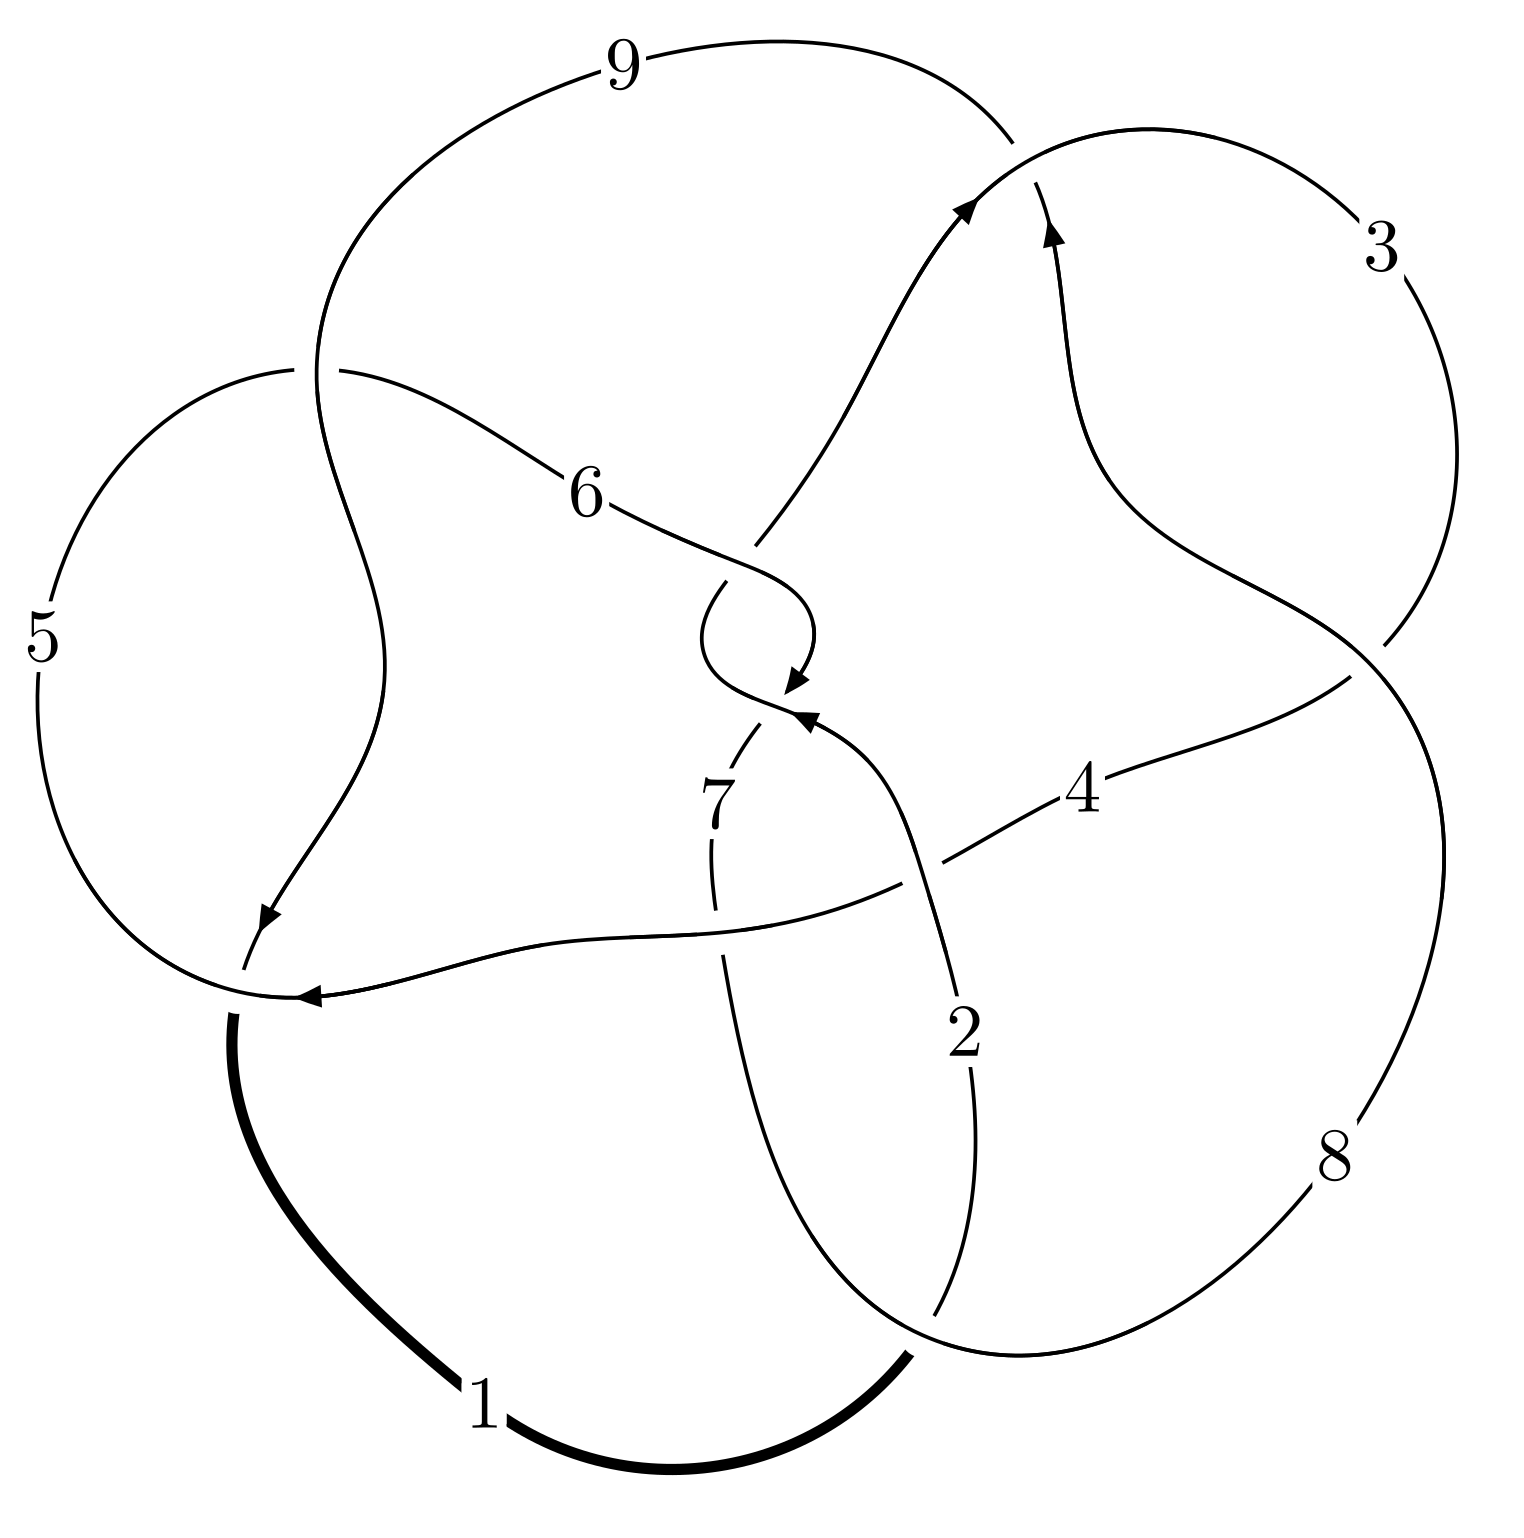
\includegraphics[width=112pt]{../../../GIT/diagram.site/Diagrams/png/84_9_49.png}\\
\ \ \ A knot diagram\footnotemark}&
\allowdisplaybreaks
\textbf{Linearized knot diagam} \\
\cline{2-2}
 &
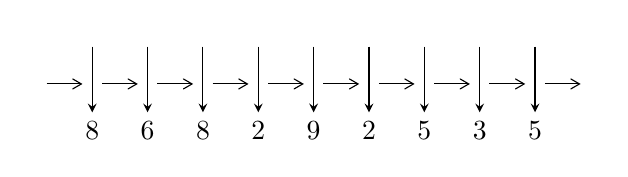
\begin{tikzpicture}[x=20pt, y=17pt]
	% nodes
	\node (C0) at (0, 0) {};
	\node (C1) at (1, 0) {};
	\node (C1U) at (1, +1) {};
	\node (C1D) at (1, -1) {8};

	\node (C2) at (2, 0) {};
	\node (C2U) at (2, +1) {};
	\node (C2D) at (2, -1) {6};

	\node (C3) at (3, 0) {};
	\node (C3U) at (3, +1) {};
	\node (C3D) at (3, -1) {8};

	\node (C4) at (4, 0) {};
	\node (C4U) at (4, +1) {};
	\node (C4D) at (4, -1) {2};

	\node (C5) at (5, 0) {};
	\node (C5U) at (5, +1) {};
	\node (C5D) at (5, -1) {9};

	\node (C6) at (6, 0) {};
	\node (C6U) at (6, +1) {};
	\node (C6D) at (6, -1) {2};

	\node (C7) at (7, 0) {};
	\node (C7U) at (7, +1) {};
	\node (C7D) at (7, -1) {5};

	\node (C8) at (8, 0) {};
	\node (C8U) at (8, +1) {};
	\node (C8D) at (8, -1) {3};

	\node (C9) at (9, 0) {};
	\node (C9U) at (9, +1) {};
	\node (C9D) at (9, -1) {5};
	\node (C10) at (10, 0) {};

	% arrows
	\draw[->,>={angle 60}]
	(C0) edge (C1) (C1) edge (C2) (C2) edge (C3) (C3) edge (C4) (C4) edge (C5) (C5) edge (C6) (C6) edge (C7) (C7) edge (C8) (C8) edge (C9) (C9) edge (C10) ;	\draw[->,>=stealth]
	(C1U) edge (C1D) (C2U) edge (C2D) (C3U) edge (C3D) (C4U) edge (C4D) (C5U) edge (C5D) (C6U) edge (C6D) (C7U) edge (C7D) (C8U) edge (C8D) (C9U) edge (C9D) ;
	\end{tikzpicture} \\
\hhline{~~} \\& 
\textbf{Solving Sequence} \\ \cline{2-2} 
 &
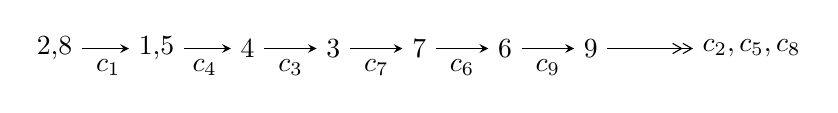
\begin{tikzpicture}[x=31pt, y=7pt]
	% node
	\node (A0) at (-1/8, 0) {2,8};
	\node (A1) at (17/16, 0) {1,5};
	\node (A2) at (17/8, 0) {4};
	\node (A3) at (25/8, 0) {3};
	\node (A4) at (33/8, 0) {7};
	\node (A5) at (41/8, 0) {6};
	\node (A6) at (49/8, 0) {9};
	\node (C1) at (1/2, -1) {$c_{1}$};
	\node (C2) at (13/8, -1) {$c_{4}$};
	\node (C3) at (21/8, -1) {$c_{3}$};
	\node (C4) at (29/8, -1) {$c_{7}$};
	\node (C5) at (37/8, -1) {$c_{6}$};
	\node (C6) at (45/8, -1) {$c_{9}$};
	\node (A7) at (8, 0) {$c_{2},c_{5},c_{8}$};

	% edge
	\draw[->,>=stealth]	
	(A0) edge (A1) (A1) edge (A2) (A2) edge (A3) (A3) edge (A4) (A4) edge (A5) (A5) edge (A6) ;
	\draw[->>,>={angle 60}]	
	(A6) edge (A7);
\end{tikzpicture} \\ 

\end{tabular} \\

\footnotetext{
The image of knot diagram is generated by the software ``\textbf{Draw programme}" developed by Andrew Bartholomew(\url{http://www.layer8.co.uk/maths/draw/index.htm\#Running-draw}), where we modified some parts for our purpose(\url{https://github.com/CATsTAILs/LinksPainter}).
}\phantom \\ \newline 
\centering \textbf{Ideals for irreducible components\footnotemark of $X_{\text{par}}$} 
 
\begin{align*}
I^u_{1}&=\langle 
b+u,\;a-1,\;u^3-3 u^2+2 u+1\rangle \\
I^u_{2}&=\langle 
b+u,\;a^2- a u+2 u+4,\;u^2+u-1\rangle \\
I^u_{3}&=\langle 
u^3-3 u^2+2 b+3 u-4,\;- u^3+2 u^2+2 a-2 u+3,\;u^4-3 u^3+5 u^2-6 u+4\rangle \\
I^u_{4}&=\langle 
b^2- b u+b+2,\;a-1,\;u^2+u-1\rangle \\
I^u_{5}&=\langle 
b+u,\;a+1,\;u^3+u^2+1\rangle \\
\\
\end{align*}
\raggedright * 5 irreducible components of $\dim_{\mathbb{C}}=0$, with total 18 representations.\\
\footnotetext{All coefficients of polynomials are rational numbers. But the coefficients are sometimes approximated in decimal forms when there is not enough margin.}
\newpage
\renewcommand{\arraystretch}{1}
\centering \section*{I. $I^u_{1}= \langle b+u,\;a-1,\;u^3-3 u^2+2 u+1 \rangle$}
\flushleft \textbf{(i) Arc colorings}\\
\begin{tabular}{m{7pt} m{180pt} m{7pt} m{180pt} }
\flushright $a_{2}=$&$\begin{pmatrix}1\\0\end{pmatrix}$ \\
\flushright $a_{8}=$&$\begin{pmatrix}0\\u\end{pmatrix}$ \\
\flushright $a_{1}=$&$\begin{pmatrix}1\\- u^2\end{pmatrix}$ \\
\flushright $a_{5}=$&$\begin{pmatrix}1\\- u\end{pmatrix}$ \\
\flushright $a_{4}=$&$\begin{pmatrix}- u+1\\- u\end{pmatrix}$ \\
\flushright $a_{3}=$&$\begin{pmatrix}- u+1\\2 u^2-3 u-1\end{pmatrix}$ \\
\flushright $a_{7}=$&$\begin{pmatrix}u\\- u^2+u\end{pmatrix}$ \\
\flushright $a_{6}=$&$\begin{pmatrix}- u^2+2 u\\- u^2+u\end{pmatrix}$ \\
\flushright $a_{9}=$&$\begin{pmatrix}- u^2+u+1\\u^2-2 u-1\end{pmatrix}$\\ \flushright $a_{9}=$&$\begin{pmatrix}- u^2+u+1\\u^2-2 u-1\end{pmatrix}$\\&\end{tabular}
\flushleft \textbf{(ii) Obstruction class $= -1$}\\~\\
\flushleft \textbf{(iii) Cusp Shapes $= 3 u^2-15$}\\~\\
\newpage\renewcommand{\arraystretch}{1}
\flushleft \textbf{(iv) u-Polynomials at the component}\newline \\
\begin{tabular}{m{50pt}|m{274pt}}
Crossings & \hspace{64pt}u-Polynomials at each crossing \\
\hline $$\begin{aligned}c_{1},c_{4},c_{7}\end{aligned}$$&$\begin{aligned}
&u^3-3 u^2+2 u+1
\end{aligned}$\\
\hline $$\begin{aligned}c_{2},c_{3},c_{5}\\c_{6},c_{8},c_{9}\end{aligned}$$&$\begin{aligned}
&u^3+2 u^2+3 u+1
\end{aligned}$\\
\hline
\end{tabular}\\~\\
\newpage\renewcommand{\arraystretch}{1}
\flushleft \textbf{(v) Riley Polynomials at the component}\newline \\
\begin{tabular}{m{50pt}|m{274pt}}
Crossings & \hspace{64pt}Riley Polynomials at each crossing \\
\hline $$\begin{aligned}c_{1},c_{4},c_{7}\end{aligned}$$&$\begin{aligned}
&y^3-5 y^2+10 y-1
\end{aligned}$\\
\hline $$\begin{aligned}c_{2},c_{3},c_{5}\\c_{6},c_{8},c_{9}\end{aligned}$$&$\begin{aligned}
&y^3+2 y^2+5 y-1
\end{aligned}$\\
\hline
\end{tabular}\\~\\
\newpage\flushleft \textbf{(vi) Complex Volumes and Cusp Shapes}
$$\begin{array}{c|c|c}  
\text{Solutions to }I^u_{1}& \I (\text{vol} + \sqrt{-1}CS) & \text{Cusp shape}\\
 \hline 
\begin{aligned}
u &= -0.324718\phantom{ +0.000000I} \\
a &= \phantom{-}1.00000\phantom{ +0.000000I} \\
b &= \phantom{-}0.324718\phantom{ +0.000000I}\end{aligned}
 & -0.674976\phantom{ +0.000000I} & -14.6840\phantom{ +0.000000I} \\ \hline\begin{aligned}
u &= \phantom{-}1.66236 + 0.56228 I \\
a &= \phantom{-}1.00000\phantom{ +0.000000I} \\
b &= -1.66236 - 0.56228 I\end{aligned}
 & -1.30745 - 9.42707 I & -7.65816 + 5.60826 I \\ \hline\begin{aligned}
u &= \phantom{-}1.66236 - 0.56228 I \\
a &= \phantom{-}1.00000\phantom{ +0.000000I} \\
b &= -1.66236 + 0.56228 I\end{aligned}
 & -1.30745 + 9.42707 I & -7.65816 - 5.60826 I\\
 \hline 
 \end{array}$$\newpage\newpage\renewcommand{\arraystretch}{1}
\centering \section*{II. $I^u_{2}= \langle b+u,\;a^2- a u+2 u+4,\;u^2+u-1 \rangle$}
\flushleft \textbf{(i) Arc colorings}\\
\begin{tabular}{m{7pt} m{180pt} m{7pt} m{180pt} }
\flushright $a_{2}=$&$\begin{pmatrix}1\\0\end{pmatrix}$ \\
\flushright $a_{8}=$&$\begin{pmatrix}0\\u\end{pmatrix}$ \\
\flushright $a_{1}=$&$\begin{pmatrix}1\\u-1\end{pmatrix}$ \\
\flushright $a_{5}=$&$\begin{pmatrix}a\\- u\end{pmatrix}$ \\
\flushright $a_{4}=$&$\begin{pmatrix}a- u\\- u\end{pmatrix}$ \\
\flushright $a_{3}=$&$\begin{pmatrix}a- u\\a u- a+u-1\end{pmatrix}$ \\
\flushright $a_{7}=$&$\begin{pmatrix}- a u+a-2 u-2\\a u- a+u\end{pmatrix}$ \\
\flushright $a_{6}=$&$\begin{pmatrix}- u-2\\a u- a+u\end{pmatrix}$ \\
\flushright $a_{9}=$&$\begin{pmatrix}- a u+a+3\\2 a u- a+2 u-2\end{pmatrix}$\\ \flushright $a_{9}=$&$\begin{pmatrix}- a u+a+3\\2 a u- a+2 u-2\end{pmatrix}$\\&\end{tabular}
\flushleft \textbf{(ii) Obstruction class $= -1$}\\~\\
\flushleft \textbf{(iii) Cusp Shapes $= 4 a u-4 a+4 u-10$}\\~\\
\newpage\renewcommand{\arraystretch}{1}
\flushleft \textbf{(iv) u-Polynomials at the component}\newline \\
\begin{tabular}{m{50pt}|m{274pt}}
Crossings & \hspace{64pt}u-Polynomials at each crossing \\
\hline $$\begin{aligned}c_{1},c_{4}\end{aligned}$$&$\begin{aligned}
&(u^2+u-1)^2
\end{aligned}$\\
\hline $$\begin{aligned}c_{2},c_{5},c_{6}\\c_{9}\end{aligned}$$&$\begin{aligned}
&(u^2- u+1)^2
\end{aligned}$\\
\hline $$\begin{aligned}c_{3},c_{8}\end{aligned}$$&$\begin{aligned}
&u^4+3 u^3+5 u^2+6 u+4
\end{aligned}$\\
\hline $$\begin{aligned}c_{7}\end{aligned}$$&$\begin{aligned}
&u^4-3 u^3+5 u^2-6 u+4
\end{aligned}$\\
\hline
\end{tabular}\\~\\
\newpage\renewcommand{\arraystretch}{1}
\flushleft \textbf{(v) Riley Polynomials at the component}\newline \\
\begin{tabular}{m{50pt}|m{274pt}}
Crossings & \hspace{64pt}Riley Polynomials at each crossing \\
\hline $$\begin{aligned}c_{1},c_{4}\end{aligned}$$&$\begin{aligned}
&(y^2-3 y+1)^2
\end{aligned}$\\
\hline $$\begin{aligned}c_{2},c_{5},c_{6}\\c_{9}\end{aligned}$$&$\begin{aligned}
&(y^2+y+1)^2
\end{aligned}$\\
\hline $$\begin{aligned}c_{3},c_{7},c_{8}\end{aligned}$$&$\begin{aligned}
&y^4+y^3-3 y^2+4 y+16
\end{aligned}$\\
\hline
\end{tabular}\\~\\
\newpage\flushleft \textbf{(vi) Complex Volumes and Cusp Shapes}
$$\begin{array}{c|c|c}  
\text{Solutions to }I^u_{2}& \I (\text{vol} + \sqrt{-1}CS) & \text{Cusp shape}\\
 \hline 
\begin{aligned}
u &= \phantom{-}0.618034\phantom{ +0.000000I} \\
a &= \phantom{-}0.30902 + 2.26728 I \\
b &= -0.618034\phantom{ +0.000000I}\end{aligned}
 & \phantom{-}3.94784 + 2.02988 I & -8.00000 - 3.46410 I \\ \hline\begin{aligned}
u &= \phantom{-}0.618034\phantom{ +0.000000I} \\
a &= \phantom{-}0.30902 - 2.26728 I \\
b &= -0.618034\phantom{ +0.000000I}\end{aligned}
 & \phantom{-}3.94784 - 2.02988 I & -8.00000 + 3.46410 I \\ \hline\begin{aligned}
u &= -1.61803\phantom{ +0.000000I} \\
a &= -0.809017 + 0.330792 I \\
b &= \phantom{-}1.61803\phantom{ +0.000000I}\end{aligned}
 & -3.94784 + 2.02988 I & -8.00000 - 3.46410 I \\ \hline\begin{aligned}
u &= -1.61803\phantom{ +0.000000I} \\
a &= -0.809017 - 0.330792 I \\
b &= \phantom{-}1.61803\phantom{ +0.000000I}\end{aligned}
 & -3.94784 - 2.02988 I & -8.00000 + 3.46410 I\\
 \hline 
 \end{array}$$\newpage\newpage\renewcommand{\arraystretch}{1}
\centering \section*{III. $I^u_{3}= \langle u^3-3 u^2+2 b+3 u-4,\;- u^3+2 u^2+2 a-2 u+3,\;u^4-3 u^3+5 u^2-6 u+4 \rangle$}
\flushleft \textbf{(i) Arc colorings}\\
\begin{tabular}{m{7pt} m{180pt} m{7pt} m{180pt} }
\flushright $a_{2}=$&$\begin{pmatrix}1\\0\end{pmatrix}$ \\
\flushright $a_{8}=$&$\begin{pmatrix}0\\u\end{pmatrix}$ \\
\flushright $a_{1}=$&$\begin{pmatrix}1\\- u^2\end{pmatrix}$ \\
\flushright $a_{5}=$&$\begin{pmatrix}\frac{1}{2} u^3- u^2+u-\frac{3}{2}\\-\frac{1}{2} u^3+\frac{3}{2} u^2-\frac{3}{2} u+2\end{pmatrix}$ \\
\flushright $a_{4}=$&$\begin{pmatrix}\frac{1}{2} u^2-\frac{1}{2} u+\frac{1}{2}\\-\frac{1}{2} u^3+\frac{3}{2} u^2-\frac{3}{2} u+2\end{pmatrix}$ \\
\flushright $a_{3}=$&$\begin{pmatrix}\frac{1}{2} u^2-\frac{1}{2} u+\frac{1}{2}\\-\frac{3}{2} u^3+\frac{7}{2} u^2-\frac{9}{2} u+4\end{pmatrix}$ \\
\flushright $a_{7}=$&$\begin{pmatrix}-\frac{3}{4} u^3+\frac{7}{4} u^2-\frac{9}{4} u+3\\\frac{1}{2} u^3-\frac{3}{2} u^2+\frac{5}{2} u-3\end{pmatrix}$ \\
\flushright $a_{6}=$&$\begin{pmatrix}-\frac{1}{4} u^3+\frac{1}{4} u^2+\frac{1}{4} u\\\frac{1}{2} u^3-\frac{3}{2} u^2+\frac{5}{2} u-3\end{pmatrix}$ \\
\flushright $a_{9}=$&$\begin{pmatrix}-\frac{1}{4} u^3+\frac{1}{4} u^2-\frac{3}{4} u+1\\\frac{1}{2} u^3-\frac{3}{2} u^2+\frac{3}{2} u-1\end{pmatrix}$\\ \flushright $a_{9}=$&$\begin{pmatrix}-\frac{1}{4} u^3+\frac{1}{4} u^2-\frac{3}{4} u+1\\\frac{1}{2} u^3-\frac{3}{2} u^2+\frac{3}{2} u-1\end{pmatrix}$\\&\end{tabular}
\flushleft \textbf{(ii) Obstruction class $= -1$}\\~\\
\flushleft \textbf{(iii) Cusp Shapes $= 2 u^3-2 u^2+2 u-10$}\\~\\
\newpage\renewcommand{\arraystretch}{1}
\flushleft \textbf{(iv) u-Polynomials at the component}\newline \\
\begin{tabular}{m{50pt}|m{274pt}}
Crossings & \hspace{64pt}u-Polynomials at each crossing \\
\hline $$\begin{aligned}c_{1}\end{aligned}$$&$\begin{aligned}
&u^4-3 u^3+5 u^2-6 u+4
\end{aligned}$\\
\hline $$\begin{aligned}c_{2},c_{6}\end{aligned}$$&$\begin{aligned}
&u^4+3 u^3+5 u^2+6 u+4
\end{aligned}$\\
\hline $$\begin{aligned}c_{3},c_{5},c_{8}\\c_{9}\end{aligned}$$&$\begin{aligned}
&(u^2- u+1)^2
\end{aligned}$\\
\hline $$\begin{aligned}c_{4},c_{7}\end{aligned}$$&$\begin{aligned}
&(u^2+u-1)^2
\end{aligned}$\\
\hline
\end{tabular}\\~\\
\newpage\renewcommand{\arraystretch}{1}
\flushleft \textbf{(v) Riley Polynomials at the component}\newline \\
\begin{tabular}{m{50pt}|m{274pt}}
Crossings & \hspace{64pt}Riley Polynomials at each crossing \\
\hline $$\begin{aligned}c_{1},c_{2},c_{6}\end{aligned}$$&$\begin{aligned}
&y^4+y^3-3 y^2+4 y+16
\end{aligned}$\\
\hline $$\begin{aligned}c_{3},c_{5},c_{8}\\c_{9}\end{aligned}$$&$\begin{aligned}
&(y^2+y+1)^2
\end{aligned}$\\
\hline $$\begin{aligned}c_{4},c_{7}\end{aligned}$$&$\begin{aligned}
&(y^2-3 y+1)^2
\end{aligned}$\\
\hline
\end{tabular}\\~\\
\newpage\flushleft \textbf{(vi) Complex Volumes and Cusp Shapes}
$$\begin{array}{c|c|c}  
\text{Solutions to }I^u_{3}& \I (\text{vol} + \sqrt{-1}CS) & \text{Cusp shape}\\
 \hline 
\begin{aligned}
u &= \phantom{-}1.30902 + 0.53523 I \\
a &= -1.059020 + 0.433013 I \\
b &= \phantom{-}1.61803\phantom{ +0.000000I}\end{aligned}
 & -3.94784 - 2.02988 I & -8.00000 + 3.46410 I \\ \hline\begin{aligned}
u &= \phantom{-}1.30902 - 0.53523 I \\
a &= -1.059020 - 0.433013 I \\
b &= \phantom{-}1.61803\phantom{ +0.000000I}\end{aligned}
 & -3.94784 + 2.02988 I & -8.00000 - 3.46410 I \\ \hline\begin{aligned}
u &= \phantom{-}0.19098 + 1.40126 I \\
a &= \phantom{-}0.059017 - 0.433013 I \\
b &= -0.618034\phantom{ +0.000000I}\end{aligned}
 & \phantom{-}3.94784 + 2.02988 I & -8.00000 - 3.46410 I \\ \hline\begin{aligned}
u &= \phantom{-}0.19098 - 1.40126 I \\
a &= \phantom{-}0.059017 + 0.433013 I \\
b &= -0.618034\phantom{ +0.000000I}\end{aligned}
 & \phantom{-}3.94784 - 2.02988 I & -8.00000 + 3.46410 I\\
 \hline 
 \end{array}$$\newpage\newpage\renewcommand{\arraystretch}{1}
\centering \section*{IV. $I^u_{4}= \langle b^2- b u+b+2,\;a-1,\;u^2+u-1 \rangle$}
\flushleft \textbf{(i) Arc colorings}\\
\begin{tabular}{m{7pt} m{180pt} m{7pt} m{180pt} }
\flushright $a_{2}=$&$\begin{pmatrix}1\\0\end{pmatrix}$ \\
\flushright $a_{8}=$&$\begin{pmatrix}0\\u\end{pmatrix}$ \\
\flushright $a_{1}=$&$\begin{pmatrix}1\\u-1\end{pmatrix}$ \\
\flushright $a_{5}=$&$\begin{pmatrix}1\\b\end{pmatrix}$ \\
\flushright $a_{4}=$&$\begin{pmatrix}b+1\\b\end{pmatrix}$ \\
\flushright $a_{3}=$&$\begin{pmatrix}b+1\\b u+u-1\end{pmatrix}$ \\
\flushright $a_{7}=$&$\begin{pmatrix}u\\b u+u\end{pmatrix}$ \\
\flushright $a_{6}=$&$\begin{pmatrix}b u+2 u\\b u+u\end{pmatrix}$ \\
\flushright $a_{9}=$&$\begin{pmatrix}- b+u\\u+1\end{pmatrix}$\\ \flushright $a_{9}=$&$\begin{pmatrix}- b+u\\u+1\end{pmatrix}$\\&\end{tabular}
\flushleft \textbf{(ii) Obstruction class $= -1$}\\~\\
\flushleft \textbf{(iii) Cusp Shapes $= 4 b u+4 u-10$}\\~\\
\newpage\renewcommand{\arraystretch}{1}
\flushleft \textbf{(iv) u-Polynomials at the component}\newline \\
\begin{tabular}{m{50pt}|m{274pt}}
Crossings & \hspace{64pt}u-Polynomials at each crossing \\
\hline $$\begin{aligned}c_{1},c_{7}\end{aligned}$$&$\begin{aligned}
&(u^2+u-1)^2
\end{aligned}$\\
\hline $$\begin{aligned}c_{2},c_{3},c_{6}\\c_{8}\end{aligned}$$&$\begin{aligned}
&(u^2- u+1)^2
\end{aligned}$\\
\hline $$\begin{aligned}c_{4}\end{aligned}$$&$\begin{aligned}
&u^4-3 u^3+5 u^2-6 u+4
\end{aligned}$\\
\hline $$\begin{aligned}c_{5},c_{9}\end{aligned}$$&$\begin{aligned}
&u^4+3 u^3+5 u^2+6 u+4
\end{aligned}$\\
\hline
\end{tabular}\\~\\
\newpage\renewcommand{\arraystretch}{1}
\flushleft \textbf{(v) Riley Polynomials at the component}\newline \\
\begin{tabular}{m{50pt}|m{274pt}}
Crossings & \hspace{64pt}Riley Polynomials at each crossing \\
\hline $$\begin{aligned}c_{1},c_{7}\end{aligned}$$&$\begin{aligned}
&(y^2-3 y+1)^2
\end{aligned}$\\
\hline $$\begin{aligned}c_{2},c_{3},c_{6}\\c_{8}\end{aligned}$$&$\begin{aligned}
&(y^2+y+1)^2
\end{aligned}$\\
\hline $$\begin{aligned}c_{4},c_{5},c_{9}\end{aligned}$$&$\begin{aligned}
&y^4+y^3-3 y^2+4 y+16
\end{aligned}$\\
\hline
\end{tabular}\\~\\
\newpage\flushleft \textbf{(vi) Complex Volumes and Cusp Shapes}
$$\begin{array}{c|c|c}  
\text{Solutions to }I^u_{4}& \I (\text{vol} + \sqrt{-1}CS) & \text{Cusp shape}\\
 \hline 
\begin{aligned}
u &= \phantom{-}0.618034\phantom{ +0.000000I} \\
a &= \phantom{-}1.00000\phantom{ +0.000000I} \\
b &= -0.19098 + 1.40126 I\end{aligned}
 & \phantom{-}3.94784 - 2.02988 I & -8.00000 + 3.46410 I \\ \hline\begin{aligned}
u &= \phantom{-}0.618034\phantom{ +0.000000I} \\
a &= \phantom{-}1.00000\phantom{ +0.000000I} \\
b &= -0.19098 - 1.40126 I\end{aligned}
 & \phantom{-}3.94784 + 2.02988 I & -8.00000 - 3.46410 I \\ \hline\begin{aligned}
u &= -1.61803\phantom{ +0.000000I} \\
a &= \phantom{-}1.00000\phantom{ +0.000000I} \\
b &= -1.30902 + 0.53523 I\end{aligned}
 & -3.94784 + 2.02988 I & -8.00000 - 3.46410 I \\ \hline\begin{aligned}
u &= -1.61803\phantom{ +0.000000I} \\
a &= \phantom{-}1.00000\phantom{ +0.000000I} \\
b &= -1.30902 - 0.53523 I\end{aligned}
 & -3.94784 - 2.02988 I & -8.00000 + 3.46410 I\\
 \hline 
 \end{array}$$\newpage\newpage\renewcommand{\arraystretch}{1}
\centering \section*{V. $I^u_{5}= \langle b+u,\;a+1,\;u^3+u^2+1 \rangle$}
\flushleft \textbf{(i) Arc colorings}\\
\begin{tabular}{m{7pt} m{180pt} m{7pt} m{180pt} }
\flushright $a_{2}=$&$\begin{pmatrix}1\\0\end{pmatrix}$ \\
\flushright $a_{8}=$&$\begin{pmatrix}0\\u\end{pmatrix}$ \\
\flushright $a_{1}=$&$\begin{pmatrix}1\\- u^2\end{pmatrix}$ \\
\flushright $a_{5}=$&$\begin{pmatrix}-1\\- u\end{pmatrix}$ \\
\flushright $a_{4}=$&$\begin{pmatrix}- u-1\\- u\end{pmatrix}$ \\
\flushright $a_{3}=$&$\begin{pmatrix}- u-1\\- u-1\end{pmatrix}$ \\
\flushright $a_{7}=$&$\begin{pmatrix}u\\u^2+u\end{pmatrix}$ \\
\flushright $a_{6}=$&$\begin{pmatrix}u^2+2 u\\u^2+u\end{pmatrix}$ \\
\flushright $a_{9}=$&$\begin{pmatrix}- u^2- u+1\\- u^2+1\end{pmatrix}$\\ \flushright $a_{9}=$&$\begin{pmatrix}- u^2- u+1\\- u^2+1\end{pmatrix}$\\&\end{tabular}
\flushleft \textbf{(ii) Obstruction class $= 1$}\\~\\
\flushleft \textbf{(iii) Cusp Shapes $= -3 u^2-3$}\\~\\
\newpage\renewcommand{\arraystretch}{1}
\flushleft \textbf{(iv) u-Polynomials at the component}\newline \\
\begin{tabular}{m{50pt}|m{274pt}}
Crossings & \hspace{64pt}u-Polynomials at each crossing \\
\hline $$\begin{aligned}c_{1},c_{4},c_{7}\end{aligned}$$&$\begin{aligned}
&u^3+u^2+1
\end{aligned}$\\
\hline $$\begin{aligned}c_{2},c_{5},c_{8}\end{aligned}$$&$\begin{aligned}
&u^3+u-1
\end{aligned}$\\
\hline $$\begin{aligned}c_{3},c_{6},c_{9}\end{aligned}$$&$\begin{aligned}
&u^3+u+1
\end{aligned}$\\
\hline
\end{tabular}\\~\\
\newpage\renewcommand{\arraystretch}{1}
\flushleft \textbf{(v) Riley Polynomials at the component}\newline \\
\begin{tabular}{m{50pt}|m{274pt}}
Crossings & \hspace{64pt}Riley Polynomials at each crossing \\
\hline $$\begin{aligned}c_{1},c_{4},c_{7}\end{aligned}$$&$\begin{aligned}
&y^3- y^2-2 y-1
\end{aligned}$\\
\hline $$\begin{aligned}c_{2},c_{3},c_{5}\\c_{6},c_{8},c_{9}\end{aligned}$$&$\begin{aligned}
&y^3+2 y^2+y-1
\end{aligned}$\\
\hline
\end{tabular}\\~\\
\newpage\flushleft \textbf{(vi) Complex Volumes and Cusp Shapes}
$$\begin{array}{c|c|c}  
\text{Solutions to }I^u_{5}& \I (\text{vol} + \sqrt{-1}CS) & \text{Cusp shape}\\
 \hline 
\begin{aligned}
u &= \phantom{-}0.232786 + 0.792552 I \\
a &= -1.00000\phantom{ +0.000000I} \\
b &= -0.232786 - 0.792552 I\end{aligned}
 & \phantom{-}5.50124 + 1.58317 I & -1.27815 - 1.10697 I \\ \hline\begin{aligned}
u &= \phantom{-}0.232786 - 0.792552 I \\
a &= -1.00000\phantom{ +0.000000I} \\
b &= -0.232786 + 0.792552 I\end{aligned}
 & \phantom{-}5.50124 - 1.58317 I & -1.27815 + 1.10697 I \\ \hline\begin{aligned}
u &= -1.46557\phantom{ +0.000000I} \\
a &= -1.00000\phantom{ +0.000000I} \\
b &= \phantom{-}1.46557\phantom{ +0.000000I}\end{aligned}
 & -4.42273\phantom{ +0.000000I} & -9.44370\phantom{ +0.000000I}\\
 \hline 
 \end{array}$$\newpage
\newpage\renewcommand{\arraystretch}{1}
\centering \section*{ VI. u-Polynomials}
\begin{tabular}{m{50pt}|m{274pt}}
Crossings & \hspace{64pt}u-Polynomials at each crossing \\
\hline $$\begin{aligned}c_{1},c_{4},c_{7}\end{aligned}$$&$\begin{aligned}
&((u^2+u-1)^4)(u^{3}-3 u^{2}+2 u+1)(u^3+u^2+1)(u^{4}-3 u^{3}+\cdots-6 u+4)
\end{aligned}$\\
\hline $$\begin{aligned}c_{2},c_{5},c_{8}\end{aligned}$$&$\begin{aligned}
&((u^2- u+1)^4)(u^3+u-1)(u^{3}+2 u^{2}+3 u+1)(u^{4}+3 u^{3}+\cdots+6 u+4)
\end{aligned}$\\
\hline $$\begin{aligned}c_{3},c_{6},c_{9}\end{aligned}$$&$\begin{aligned}
&((u^2- u+1)^4)(u^3+u+1)(u^{3}+2 u^{2}+3 u+1)(u^{4}+3 u^{3}+\cdots+6 u+4)
\end{aligned}$\\
\hline
\end{tabular}\newpage\renewcommand{\arraystretch}{1}
\centering \section*{ VII. Riley Polynomials}
\begin{tabular}{m{50pt}|m{274pt}}
Crossings & \hspace{64pt}Riley Polynomials at each crossing \\
\hline $$\begin{aligned}c_{1},c_{4},c_{7}\end{aligned}$$&$\begin{aligned}
&(y^2-3 y+1)^4(y^3-5 y^2+10 y-1)(y^3- y^2-2 y-1)\\
&\cdot(y^4+y^3-3 y^2+4 y+16)
\end{aligned}$\\
\hline $$\begin{aligned}c_{2},c_{3},c_{5}\\c_{6},c_{8},c_{9}\end{aligned}$$&$\begin{aligned}
&(y^2+y+1)^4(y^3+2 y^2+y-1)(y^3+2 y^2+5 y-1)\\
&\cdot(y^4+y^3-3 y^2+4 y+16)
\end{aligned}$\\
\hline
\end{tabular}
\vskip 2pc
\end{document}